\documentclass[aspectratio=169,10pt]{beamer}

\usetheme{Madrid}
\usecolortheme{default}
\usepackage{graphicx}
\usepackage{booktabs}
\usepackage{amsmath}
\usepackage{tikz}
\usepackage{hyperref}
\usepackage{xcolor}
\usepackage{multicol}
\usetikzlibrary{shapes.geometric, arrows.meta, positioning, fit}

% Custom colors
\definecolor{darkblue}{RGB}{33, 37, 41}
\definecolor{lightblue}{RGB}{66, 133, 244}
\definecolor{greencolor}{RGB}{76, 175, 80}
\definecolor{warnred}{RGB}{211, 47, 47}
\definecolor{warnorg}{RGB}{245, 124, 0}

\setbeamercolor{structure}{fg=darkblue}
\setbeamercolor{frametitle}{bg=lightblue!10,fg=darkblue}

% Remove navigation symbols
\setbeamertemplate{navigation symbols}{}

\title{Satellite NDVI Forecasting with\\Growth Curve Regression}
\subtitle{Partial Results \& Model Diagnosis}
\author{Antonio H. X. da Silva}
\date{February 2026}
\institute{NOVA IMS}

\begin{document}

% =============================================================================
% TITLE SLIDE
% =============================================================================
\begin{frame}
    \titlepage
\end{frame}

% =============================================================================
% OUTLINE
% =============================================================================
\begin{frame}{Outline}
    \tableofcontents
\end{frame}

% =============================================================================
\section{Recap}
% =============================================================================

\begin{frame}{Project Recap}
    \begin{columns}
        \column{0.5\textwidth}
        \textbf{Objective}
        \begin{itemize}
            \item Forecast vegetation dynamics over 100-day horizon
            \item Input: 10 Sentinel-2 frames (50 days)
            \item Output: 20 predicted delta frames (100 days)
            \item Parametric growth curve decoder for interpretability
        \end{itemize}
        
        \vspace{0.4cm}
        \textbf{Data}
        \begin{itemize}
            \item GreenEarthNet dataset (Sentinel-2 + E-OBS)
            \item 4 spectral bands: B02, B03, B04, B8A
            \item ESA WorldCover land classification
        \end{itemize}
        
        \column{0.5\textwidth}
        \begin{center}
            \includegraphics[width=\textwidth]{images/ModelArchitecture.drawio.png}
        \end{center}
        \vspace{0.2cm}
        \begin{block}{Growth Curve Formula}
            $\delta(t) = A \cdot (1 - e^{-\lambda \cdot T \cdot t \cdot \text{adj}(t)}) + B$
        \end{block}
    \end{columns}
\end{frame}

% =============================================================================
\section{Dataset Characteristics}
% =============================================================================

\begin{frame}{Dataset Statistics}
    \begin{columns}
        \column{0.45\textwidth}
        \begin{table}
            \centering
            \small
            \begin{tabular}{lcc}
                \toprule
                \textbf{Metric} & \textbf{Train} & \textbf{Val} \\
                \midrule
                Samples & 14213 & 952 \\
                Input Frames & 10 & 10 \\
                Output Frames & 20 & 20 \\
                Image Size & 128$\times$128 & 128$\times$128 \\
                Spectral Bands & 4 & 4 \\
                \textbf{Cloud Cover} & \textbf{31.8\%} & \textcolor{warnred}{\textbf{50.5\%}} \\
                \bottomrule
            \end{tabular}
        \end{table}
        
        \vspace{0.3cm}
        \begin{alertblock}{Cloud Coverage Disparity}
            Validation set has \textbf{$\sim$1.6$\times$ more cloud coverage} than training --- fewer valid pixels for evaluation.
        \end{alertblock}
        
        \column{0.55\textwidth}
        \begin{center}
            \includegraphics[width=\textwidth]{images/material/cloud_coverage.png}
        \end{center}
    \end{columns}
\end{frame}

% =============================================================================
\section{Model Results}
% =============================================================================

\begin{frame}{Per-Band Error Metrics}
    \begin{columns}
        \column{0.4\textwidth}
        \begin{table}
            \centering
            \begin{tabular}{lcc}
                \toprule
                \textbf{Band} & \textbf{MAE} & \textbf{RMSE} \\
                \midrule
                B02 (Blue) & 0.031 & 0.048 \\
                B03 (Green) & 0.031 & 0.048 \\
                B04 (Red) & 0.039 & 0.058 \\
                \textcolor{warnred}{B8A (NIR)} & \textcolor{warnred}{0.071} & \textcolor{warnred}{0.093} \\
                \midrule
                \textbf{Overall} & \textbf{0.043} & \textbf{0.062} \\
                \bottomrule
            \end{tabular}
            \caption{Delta prediction errors}
        \end{table}
        
        \vspace{0.2cm}
        \textbf{Observations}
        \begin{itemize}
            \item NIR has \textbf{2$\times$} the error of visible bands
            \item NIR is the most dynamic vegetation band
            \item Critical for NDVI computation
        \end{itemize}
        
        \column{0.6\textwidth}
        \begin{center}
            \includegraphics[width=\textwidth]{images/results/temporal_error.png}
        \end{center}
        \footnotesize \textit{Error increases monotonically with forecast horizon, dominated by NIR band error.}
    \end{columns}
\end{frame}

\begin{frame}{Temporal Error: NDVI Metrics}
    \begin{columns}
        \column{0.5\textwidth}
        \begin{center}
            \includegraphics[width=\textwidth]{images/results/error_analysis/temporal_error_rmse.png}
        \end{center}
        
        \column{0.5\textwidth}
        \begin{center}
            \includegraphics[width=\textwidth]{images/results/error_analysis/temporal_error_nse.png}
        \end{center}
    \end{columns}
    
    \vspace{0.3cm}
    \begin{columns}
        \column{0.5\textwidth}
        \begin{itemize}
            \item RMSE grows from 0.146 to 0.229
            \item Steepest degradation in first 30 days
        \end{itemize}
        
        \column{0.5\textwidth}
        \begin{itemize}
            \item NSE starts at \textbf{0.636} (day 1) but drops to \textbf{0.117} (day 50)
            \item Model tracks short-range dynamics reasonably well 
        \end{itemize}
    \end{columns}
\end{frame}

\begin{frame}{Prediction Comparison: Reflectance}
    \begin{center}
        \includegraphics[width=0.85\textwidth]{images/predictions/sample_0000_reflectance.png}
    \end{center}
    \vspace{-0.2cm}
    \footnotesize \textit{Top rows: ground truth reflectance. Bottom rows: predicted reflectance. Model captures broad spatial patterns but produces monotonic changes over time.}
\end{frame}

\begin{frame}{NDVI Comparison: True vs. Predicted}
    \begin{center}
        \includegraphics[width=0.9\textwidth]{images/results/ndvi_comparison.png}
    \end{center}
    \vspace{-0.2cm}
    \footnotesize \textit{NDVI tracks well at early steps (t=5, t=25) but diverges at later steps (t=75, t=100).}
\end{frame}

\begin{frame}{Error by Land Cover Class}
    \begin{columns}
        \column{0.55\textwidth}
        \begin{center}
            \includegraphics[width=\textwidth]{images/results/error_analysis/landcover_error.png}
        \end{center}
        
        \column{0.45\textwidth}
        \textbf{Key Findings}
        \begin{itemize}
            \item \textbf{Snow/ice} has the highest NDVI RMSE ($\sim$0.55) --- extreme reflectance values poorly handled
            \item \textbf{Water} and \textbf{Shrubland} follow at $\sim$0.35
            \item \textbf{Cropland} and \textbf{Built-up} have the lowest error ($\sim$0.22--0.25) --- more spectrally stable
            \item Vegetation classes (\textbf{Tree cover}, \textbf{Grassland}, \textbf{Shrubland}) cluster around 0.30--0.35
        \end{itemize}
        
        \begin{block}{Implication}
            Errors are distributed across all classes, not restricted to dynamic vegetation.
        \end{block}
    \end{columns}
\end{frame}

% =============================================================================
\section{Vegetation Score Analysis}
% =============================================================================

\begin{frame}{Vegetation Score: Benchmark Comparison}
    \begin{table}
        \centering
        \begin{tabular}{lccc}
            \toprule
            \textbf{Model} & \textbf{Parameters} & \textbf{Type} & \textbf{Veg. Score$\uparrow$} \\
            \midrule
            ConvLSTM & $\sim$2M & RNN-based & 0.21 \\
            SGED-ConvLSTM & $\sim$3M & RNN-based & 0.24 \\
            PredRNN & $\sim$24M & Video Pred. & 0.19 \\
            SimVP & $\sim$22M & Video Pred. & 0.22 \\
            Earthformer & $\sim$12M & Transformer & 0.28 \\
            \textbf{Contextformer} & \textbf{6M} & \textbf{Transformer} & \textbf{0.31} \\
            \midrule
            \textcolor{warnred}{\textbf{Ours (Growth Curve Reg.)}} & \textcolor{warnred}{$\leq$600K} & \textcolor{warnred}{RNN-Based} & \textcolor{warnred}{\textbf{Negative values}} \\
            \bottomrule
        \end{tabular}
        \caption{GreenEarthNet IID validation. Literature scores from Benson et al., CVPR 2024.}
    \end{table}
    
    \vspace{0.2cm}
    \begin{columns}
        \column{0.5\textwidth}
        \textbf{Current Gap}
        \begin{itemize}
            \item Current: far below the 0.0 threshold
            \item Target: $\geq$ 0.31 (match Contextformer)
        \end{itemize}
        \column{0.5\textwidth}
        \textbf{Current result}
        \begin{itemize}
            \item Per-step NSE is positive (0.636 at step 1)
            \item Model \textit{does learn signal}, but it degrades fast
        \end{itemize}
    \end{columns}
\end{frame}

% =============================================================================
\section{Root Cause Diagnosis}
% =============================================================================

\begin{frame}{Root Cause \#1: Monotonic Growth Curve}
    \begin{columns}
        \column{0.55\textwidth}
        \textbf{The Problem}
        
        The growth curve formula is a \textbf{saturating exponential}:
        \begin{equation*}
            \delta(t) = A \cdot \underbrace{(1 - e^{-\lambda \cdot T \cdot t \cdot \text{adj}(t)})}_{\text{monotonic saturation}} + B
        \end{equation*}
        
        \begin{itemize}
            \item Can only model \textbf{monotonic} increase or decrease toward a plateau
            \item \textbf{Cannot capture}: seasonal cycles, growth followed by senescence, fluctuations
            \item Over a 100-day horizon, vegetation NDVI may rise \textit{then} fall --- impossible with this curve
        \end{itemize}
        
        \column{0.45\textwidth}
        \begin{center}
        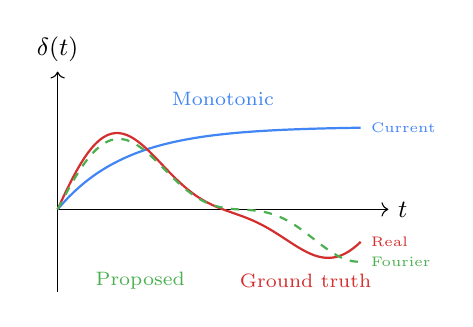
\begin{tikzpicture}[scale=0.7]
            \draw[->] (0,0) -- (6,0) node[right] {\small $t$};
            \draw[->] (0,-1.5) -- (0,2.5) node[above] {\small $\delta(t)$};
            
            % Monotonic curve (what model can do)
            \draw[thick, lightblue, domain=0:5.5, samples=80] 
                plot (\x, {1.5*(1-exp(-0.8*\x))}) node[right] {\tiny Current};
            
            % Real vegetation (what reality looks like)
            \draw[thick, warnred, domain=0:5.5, samples=80] 
                plot (\x, {1.5*sin(60*\x) * exp(-0.15*\x) + 0.3*sin(120*\x)}) node[right] {\tiny Real};
            
            % Fourier harmonics (proposed solution)
            \draw[thick, greencolor, dashed, domain=0:5.5, samples=80] 
                plot (\x, {1.2*sin(55*\x) * exp(-0.1*\x) + 0.4*sin(110*\x)}) node[right] {\tiny Fourier};
            
            % Labels
            \node[lightblue, font=\scriptsize] at (3.0, 2.0) {Monotonic};
            \node[warnred, font=\scriptsize] at (4.5, -1.3) {Ground truth};
            \node[greencolor, font=\scriptsize] at (1.5, -1.3) {Proposed};
        \end{tikzpicture}
        \end{center}
        
        \vspace{0.3cm}
        \begin{alertblock}{Primary Limitation}
            This is the \textbf{most critical} architectural issue. NSE drops from 0.636$\to$0.117 as the model cannot track non-monotonic dynamics.
        \end{alertblock}
    \end{columns}
\end{frame}

\begin{frame}{Root Cause \#2: Weather Adjustment Flaws}
    \begin{columns}
        \column{0.55\textwidth}
        \textbf{Three Issues with Weather and Time Adjustment}
        \begin{enumerate}
            \item \textbf{Temporal collapse}: per-step weather features $(B, T, 21)$ are averaged $\to$ $(B, 32)$, losing when specific events (drought, frost) occur
            \item \textbf{Spatially uniform}: output is $(B, T)$ --- a single scalar per timestep, broadcast to all $(H, W)$ pixels identically
            \item \textbf{Disconnected from curve}: adjustment only scales effective time $t \cdot \text{adj}(t)$, it cannot change the \textit{shape} of the growth curve
        \end{enumerate}
        
        \column{0.45\textwidth}
        \textbf{Current Pipeline}
        \begin{equation*}
            \underbrace{w(t)}_{\text{weather}} \xrightarrow{\text{mean}} \underbrace{\text{adj}(t)}_{\mathbb{R}^{(B,T)}} \xrightarrow{\times t} \delta(t)
        \end{equation*}
        
        \vspace{0.5cm}
        \begin{alertblock}{Consequence}
            A rainy week vs.\ a dry week in August produces nearly the same curve shape -- only stretched or compressed in time.
        \end{alertblock}
    \end{columns}
\end{frame}


% =============================================================================
\section{Next Steps (March 2026)}
% =============================================================================

\begin{frame}{Proposed: Fourier Harmonics Decoder}
    \textbf{Replace the monotonic growth curve with a sum of harmonics} --- a natural fit for vegetation phenology.
    
    \vspace{0.3cm}
    \begin{columns}
        \column{0.5\textwidth}
        \begin{block}{Proposed Formula}
            \vspace{-0.2cm}
            \begin{equation*}
                \delta(t) = \sum_{k=1}^{K} \left[ a_k \cos(k \omega t) + b_k \sin(k \omega t) \right]
            \end{equation*}
        \end{block}
    
        \begin{itemize}
            \item $a_k, b_k$: amplitude coefficients predicted per pixel per band by the encoder
            \item $\omega = 2\pi / P$: base angular frequency (linked to the forecast period)
            \item $K$: number of harmonics (controls expressiveness)
        \end{itemize}
        
        
        \column{0.45\textwidth}
        
        \textbf{Why harmonics fit phenology}:
        \begin{itemize}
            \item Vegetation \textbf{naturally oscillates}: growth $\to$ senescence $\to$ dormancy
            \item $K{=}1$: captures the dominant seasonal trend
            \item $K{=}2{-}3$: adds sub-seasonal detail (rapid greening, drought dips)
            \item Fourier basis is \textbf{orthogonal} --- each harmonic captures independent variation
        \end{itemize}
    \end{columns}
\end{frame}

\begin{frame}{Fourier Harmonics: Fitting Different Vegetation Dynamics}
    \begin{columns}
        \column{0.5\textwidth}
        \begin{center}
        \textbf{Grassland: rapid growth-senescence}
        \vspace{0.2cm}
        
        \begin{tikzpicture}[scale=0.9]
            \draw[->] (0,0) -- (6,0) node[right] {\small $t$ (days)};
            \draw[->] (0,-1.8) -- (0,2.5) node[above] {\small $\delta(t)$};
            \draw[thick, greencolor, domain=0:5.5, samples=80] 
                plot (\x, {1.2*sin(70*\x) + 0.5*cos(35*\x) - 0.3*sin(140*\x)});
            \node[greencolor, font=\footnotesize] at (3, 2) {$a_1{=}1.2,\; a_2{=}0.5,\; b_3{=}{-}0.3$};
        \end{tikzpicture}
        \end{center}
        
        \vspace{0.3cm}
        \footnotesize
        High-amplitude harmonics $\to$ strong oscillation $\to$ fast green-up followed by senescence over the 100-day horizon.
        
        \column{0.5\textwidth}
        \begin{center}
        \textbf{Forest canopy: slow, stable trend}
        \vspace{0.2cm}
        
        \begin{tikzpicture}[scale=0.9]
            \draw[->] (0,0) -- (6,0) node[right] {\small $t$ (days)};
            \draw[->] (0,-1.8) -- (0,2.5) node[above] {\small $\delta(t)$};
            \draw[thick, lightblue, domain=0:5.5, samples=80] 
                plot (\x, {0.4*sin(70*\x + 25) + 0.15*cos(35*\x + 15) + 0.08*sin(140*\x)});
            \node[lightblue, font=\footnotesize] at (3, 2) {$a_1{=}0.4,\; a_2{=}0.15,\; b_3{=}0.08$};
        \end{tikzpicture}
        \end{center}
        
        \vspace{0.3cm}
        \footnotesize
        Small coefficients $\to$ gentle oscillation $\to$ stable canopy with minimal change, different phase from grassland.
    \end{columns}
    
    \vspace{0.3cm}
    \centering
    \footnotesize \textit{The encoder learns different $(a_k, b_k)$ per pixel --- the harmonics naturally adapt to each land cover type.}
\end{frame}

\begin{frame}{Proposed: Weather \& DOY Conditioning MLP}
    \textbf{Goal}: scale and shift the base Fourier coefficients according to weather conditions and time of year.
    
    \vspace{0.3cm}
    \begin{columns}
        \column{0.5\textwidth}
        \textbf{Step 1: Per-step weather encoding}
        
        Process each forecast timestep independently (no temporal averaging):
        \begin{equation*}
            h_w(t) = \text{MLP}\bigl(w(t)\bigr) \in \mathbb{R}^{(B, T, d)}
        \end{equation*}
        
        \textbf{Step 2: Inject DOY context}
        
        \begin{equation*}
            h(t) = \bigl[h_w(t) \;\|\; \cos(\omega_{\text{doy}} \cdot t) \;\|\; \sin(\omega_{\text{doy}} \cdot t)\bigr]
        \end{equation*}
        
        \column{0.5\textwidth}
        \textbf{Step 3: Predict scale \& shift per harmonic}
        
        For each harmonic $k$, output a scaling factor $\gamma_k$ and a shift $\beta_k$:
        \begin{equation*}
            \gamma_k(t),\; \beta_k(t) = \text{Linear}\bigl(h(t)\bigr)
        \end{equation*}
        
        \textbf{Step 4: Modulate Fourier coefficients}
        \begin{align*}
            \tilde{a}_k(t) = \gamma_k^a(t) \cdot a_k + \beta_k^a(t) \\
            \tilde{b}_k(t) = \gamma_k^b(t) \cdot b_k + \beta_k^b(t)
        \end{align*}
    \end{columns}
    
    \vspace{0.3cm}
    \begin{block}{vs.\ Current Design}
        Current MLP averages all weather into a single scalar that only stretches time.\\
        New MLP preserves per-step weather and directly modulates each harmonic's amplitude and phase.
    \end{block}
\end{frame}

% \begin{frame}{Weather \& DOY Conditioning MLP --- Architecture}
%     \begin{columns}
%         \column{0.5\textwidth}
%         \begin{center}
%         \begin{tikzpicture}[
%             node distance=0.8cm,
%             box/.style={rectangle, draw, rounded corners, minimum width=3.2cm, minimum height=0.8cm, font=\small, align=center},
%             arr/.style={->, >=stealth, thick}
%         ]
%             \node[box, fill=lightblue!20] (weather) {Weather $w(t)$\\$(B, T, 21)$};
%             \node[box, fill=lightblue!20, right=0.8cm of weather] (doy) {DOY phase\\$(\cos, \sin)$};
%             \node[box, fill=yellow!20, below=of weather] (mlp1) {Per-step MLP\\$(B, T, d)$};
%             \node[box, fill=yellow!20, below=of mlp1] (concat) {Concat $[h_w \| \text{DOY}]$};
%             \node[box, fill=greencolor!20, below=of concat] (gamma) {Scale \& Shift\\$\gamma_k(t), \beta_k(t)$};
%             \node[box, fill=warnorg!15, below=of gamma] (modulate) {Modulate $a_k, b_k$\\per pixel, per step};
            
%             \draw[arr] (weather) -- (mlp1);
%             \draw[arr] (doy) |- (concat);
%             \draw[arr] (mlp1) -- (concat);
%             \draw[arr] (concat) -- (gamma);
%             \draw[arr] (gamma) -- (modulate);
%         \end{tikzpicture}
%         \end{center}
        
%         \column{0.5\textwidth}
%         \textbf{What each block does}:
%         \begin{itemize}
%             \item \textcolor{lightblue}{\textbf{Weather input}}: E-OBS features per forecast step (temperature, precipitation, radiation, etc.)
%             \item \textcolor{yellow!70!black}{\textbf{Per-step MLP}}: encodes weather
%             \item \textcolor{yellow!70!black}{\textbf{Concat}}: injects calendar position (DOY)
%             \item \textcolor{greencolor}{\textbf{Scale \& Shift}}: predicts $\gamma_k, \beta_k$ for each of $K{=}3$ harmonics
%             \item \textcolor{warnorg}{\textbf{Modulate}}: scales and shifts the base Fourier coefficients from the encoder
%         \end{itemize}
        
%         \begin{block}{Parameter Count}
%             $K{=}3$: $6$ base coefficients/pixel/band + conditioning MLP $\approx$ 8K params.
%         \end{block}
%     \end{columns}
% \end{frame}

\begin{frame}{Timeline: Next Month}
    \begin{columns}
        \column{0.5\textwidth}
        \textbf{Week 1--2: Architecture Improvements}
        \begin{enumerate}
            \item Replace monotonic growth curve with \textbf{Weather-Conditioned Fourier} decoder
            \item Per-step FiLM conditioning from weather MLP (no temporal collapse)
            \item $K{=}3$ harmonics (6 base params/pixel/band)
        \end{enumerate}
        
        \column{0.5\textwidth}
        \textbf{Week 3: Retraining \& Validation}
        \begin{enumerate}
            \setcounter{enumi}{3}
            \item Retrain on full GreenEarthNet dataset (23,816 cubes, $\sim$48h)
            \item Evaluate on \texttt{val\_chopped} and OOD splits
            \item Benchmark against Contextformer
        \end{enumerate}
        
        \vspace{0.3cm}
        \textbf{Week 4: Writing Preparation}
        \begin{enumerate}
            \setcounter{enumi}{6}
            \item Generate final figures for results chapter
            \item Interpretability: visualize learned harmonics and FiLM weights
            \item Finish writing results and discussion chapter
        \end{enumerate}
    \end{columns}
\end{frame}

% =============================================================================
% REFERENCES
% =============================================================================
\begin{frame}{References}
    \footnotesize
    \begin{enumerate}
        \item \textbf{Benson, V., Robin, C., Requena-Mesa, C., et al.} (2024). \\
        \textit{Multi-modal learning for geospatial vegetation forecasting}. \\
        Proceedings of the IEEE/CVF Conference on Computer Vision and Pattern Recognition (CVPR). \\
        \textcolor{lightblue}{\url{https://arxiv.org/abs/2303.16198}}
        
        \vspace{0.3cm}
        \item \textbf{Pellicer-Valero, O. J., Robin, C., \& Reichstein, M.} (2024). \\
        \textit{Explainable Earth Surface Forecasting Under Extreme Events}. \\
        Earth's Future, 12, e2024EF005446. \\
        \textcolor{lightblue}{\url{https://doi.org/10.1029/2024EF005446}}


        \vspace{0.3cm}
        \item \textbf{Perez, E., Strub, F., de Vries, H., Dumoulin, V., \& Courville, A.} (2017). \\
        \textit{FiLM: Visual Reasoning with a General Conditioning Layer}. \\
        AAAI 2018. arXiv:1709.07871. \\
        \textcolor{lightblue}{\url{http://arxiv.org/abs/1709.07871}}

        \vspace{0.3cm}
        \item \textbf{Negrón Juárez, R. I., \& Liu, W. T.} (2001). \\
        \textit{FFT analysis on NDVI annual cycle and climatic regionality in Northeast Brazil}. \\
        International Journal of Climatology, 21(14), 1803--1820. \\
        \textcolor{lightblue}{\url{https://doi.org/10.1002/joc.639}}

    \end{enumerate}
\end{frame}

% =============================================================================
% THANK YOU
% =============================================================================
\begin{frame}
    \centering
    \Huge Thank You!
    
    \vspace{1cm}
    \normalsize Questions?
\end{frame}

\end{document}
